\section{Problem description}
有限状态自动机(FSM "finite state machine" 或者FSA "finite state automaton" )是为研究有限内存的计算过程和某些语言类而抽象出的一种计算模型。有限状态自动机拥有有限数量的状态,每个状态可以迁移到零个或多个状态,输入字串决定执行哪个状态的迁移。有限状态自动机可以表示为一个有向图。有限状态自动机是自动机理论的研究对象。 
\subsection{定义}
有限状态自动机(FA—finite automaton)是一个五元组:
\begin{itemize}
    \item M=(Q, Σ, δ, q0, F), 其中:
    \item Q——状态的非空有穷集合。
    \item q$\in$Q,q称为M的一个状态。
    \item Σ——输入字母表。
    \item δ——状态转移函数,有时又叫作状态转换函数或者移动函数,δ:Q×Σ→Q,δ(q,a)=p。
    \item q0——M的开始状态,也可叫作初始状态或启动状态。q0 $\in$  Q。
    \item F——M的终止状态集合。F被Q包含。任给q $\in$ F,q称为M的终止状态。
    非确定有限状态自动机(NFA)与确定有限状态自动机(DFA)的唯一区别是它们的转移函数不同。确定有限状态自动机对每一个可能的输入只有一个状态的转移。非确定有限状态自动机对每一个可能的输入可以有多个状态转移,接受到输入时从这多个状态转移中非确定地选择一个。下图是一个非确定性有限状态自动机(NFA)的例子:    
\end{itemize}

\begin{figure}[htbp]	% 浮动
    \centering
    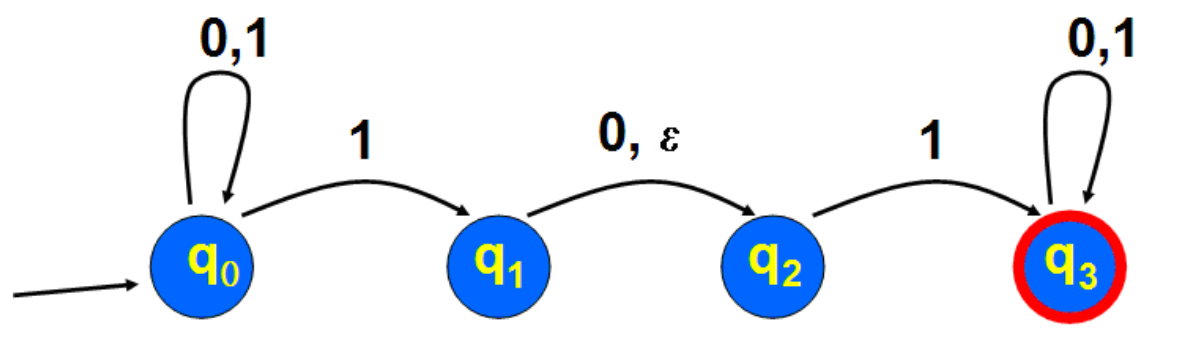
\includegraphics[width=1\linewidth]{Figure/question.png}
    \caption{一个NFA的图文表示}
    \label{fig:figure1latexintro}
\end{figure}
\subsection{状态转移表}
转移函数δ定义自下列状态转移表1。表示状态集合的子集合,采用二进制(特征)串的方式,一个子集中包含该状态,对应的特征串就为1,否则为0,比如上面状态集合的子集{q0q1q2},其特征串就是0111,而子集{q0},其特征串就是0001。将对应的特征串转换为十进制的数字,得到转移函数δ, 如表2:
\begin{figure}[htbp]
	\centering
    \subfigure[表1\#1]{
        \label{fig:sub1}		
		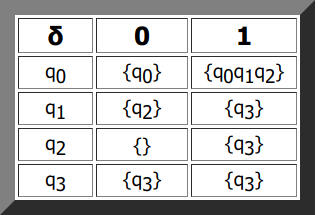
\includegraphics[width=0.45\textwidth]{Figure/table1.png}
    }
    \subfigure[表2\#2]
	{
		\label{fig:sub2}		
		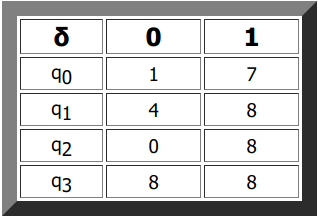
\includegraphics[width=0.45\textwidth]{Figure/table2.png}
	}
	\caption{转移函数δ表格描述}
	\label{fig:subfigure}
\end{figure}
你的任务,是要将一个给定的NFA转换为一个完全等价的DFA(有限状态自动机等价的意思是识别相同的语言)。这里我们约定自动机识别的字符集为{0,1},初始状态集合为Q0,状态集为{q0,q1,…,qn-1}。

\subsection{Input}
输入第一行只有一个正整数t,表示有t个测试数据(意味着t个NFA)t≤10;
对于每组测试数据(每个NFA),首先是3个正整数n,Q0,f,分别表示状态数、起始状态集合和接受状态集合的特征串对应的整数。n≤10;Q0,f < 2n;
接下来两行是NFA的转移函数矩阵,第一行是每个状态在输入为0的状态转移情况,用特征串对应的整数表示;第二行是每个状态在输入为1的状态转移情况。


\subsection{Output}
对于每个NFA,输出四行表示与之等价的DFA。输出格式如下:
第一行3个空格隔开的整数a b c,分别表示DFA的状态数,接受状态数,起始状态的编号(从0开始对状态编号)。要求 a < 65536。
b,c ≤ a 第二行b个空格分隔的整数,表示每个接收状态的编号,每个编号的值一定在[0,a)之间。
第三行、第四行每行a个空格分隔的整数,表示DFA的转移函数矩阵,第三行第i个值ui表示状态转移函数的一项δ(qi,0)→ui,第四行第i个值vi表示状态转移函数的一项δ(qi,1)→vi,,每个ui,vi的值一定在[0,a)之间。

\subsection{Sample Input}

\noindent1
\\4 1 8
\\1 4 0 8
\\7 8 8 8
\subsection{Sample Output}
\noindent16 8 1
\\8 9 10 11 12 13 14 15
\\0 1 4 5 0 1 4 5 8 9 12 13 8 9 12 13
\\0 7 8 15 8 15 8 15 8 15 8 15 8 15 8 15
\subsection{Judge Tips}
样例中的NFA如图一所示
与某个NFA等价的DFA不一定是唯一的,比如和图一等价的DFA可以是样例的解答,也可以是如下的DFA
\\4 1 0
\\3
\\0 2 0 3
\\1 3 3 3
\\本题会使用special judge,只要是符合条件的解答都可以接受(Accept)。